\noindent
The healthcare systems of the future will be highly decentralised, integrating home-, work- and environment-based monitoring into the hospital diagnostic systems, thus reducing costs and travel-associated risks while allowing patients to get better medical treatment (Figure~\ref{fig:dataExch}). As a consequence, medical data will need to be collected from a variety of sources and exchanged in a variety of ways, including over public networks that cannot be implicitly trusted. At the same time, we have more and more strict regulations about ownership and access rights for the patient data. Trans-national standards for data protection, such as GDPR~\cite{gdpr}, will need to be combined with local regulations, giving very strict rules about who is allowed to access what data. Complying with these rules while, at the same time, facilitating data exchange and analytics in much more distributed way will be the main challenge for the modern healtcare systems.  

\begin{figure}[h!]
    \centering
    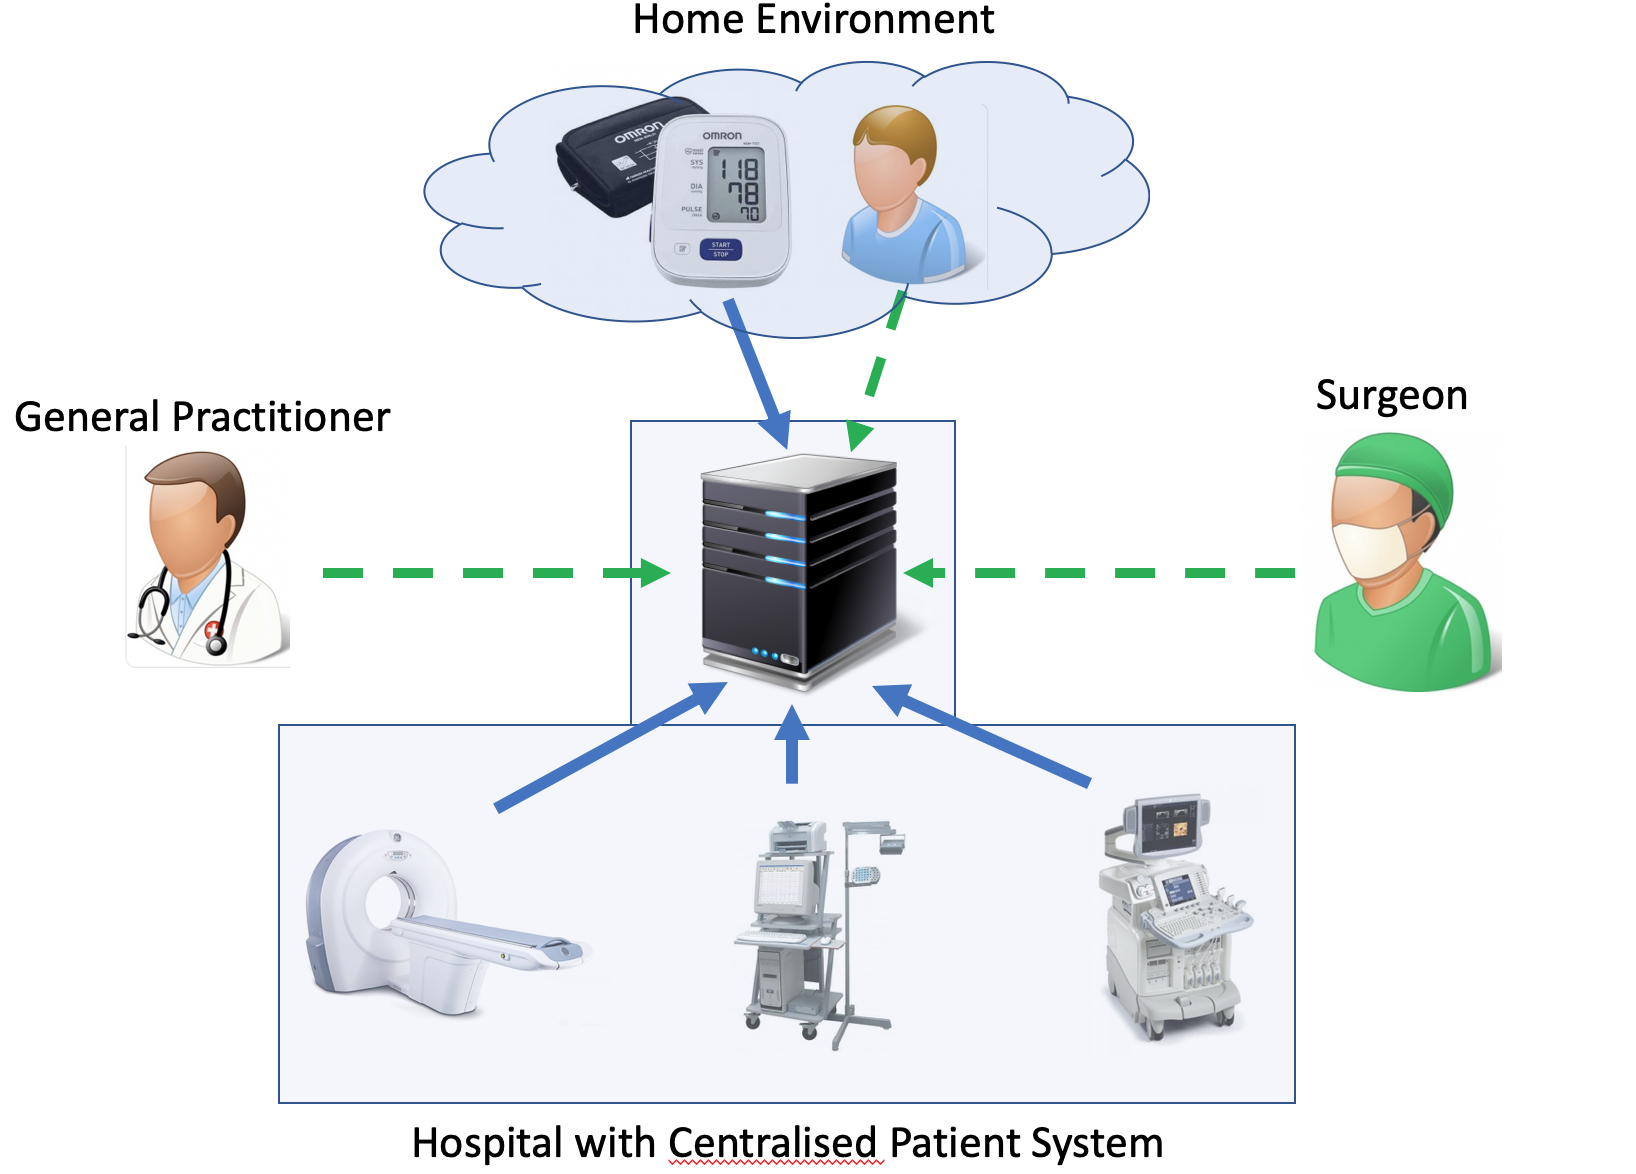
\includegraphics[scale=0.3]{images/DataExchange.png}
    \caption{Data Exhcange in Modern Healthcare Systems}
    \label{fig:dataExch}
\end{figure}



\subsection*{Notes}

Here are the items from the call for Healthcare Data and some comments/notes:
\begin{enumerate}
\item 
\emph{Health data collection and analysis:}
We have a lot of basis on this, we are clearly in both collection analytics.

\item 
\emph{Problems in health data processing:}
We have some data processing aspects, so this is also strong for us.

\item 
\emph{Protection and security of personal health data:}
We have this conceptually, and also concrete connections to GDPR.

\item 
\emph{Electronic health records and standards:}
Exactly what we're doing for the first parts, standards not so clear?
\end{enumerate}



